\chapter{Diseño de casos de prueba}
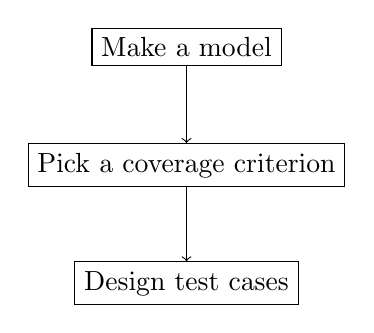
\begin{tikzpicture}[node distance=1.5cm]
   \node (model) [rectangle, draw] {Make a model};
   \node (coverage) [rectangle, draw, below of=model] {Pick a coverage criterion};
   \node (testcases) [rectangle, draw, below of=coverage] {Design test cases};

   \draw [->] (model) -- (coverage);
   \draw [->] (coverage) -- (testcases);
\end{tikzpicture}

\section{Modelos}
\note{Recuerda que el SUT (System under test) es el sistema bajo prueba.}

\subsection{Clases de equivalencia}

Se modela el input domain, y para ello se utilizan clases de equivalencia.
Es importante notar que las clases de equivalencia son una asunción, y no una verdad absoluta, pueden ser erróneas.
\begin{paracol}{2}
   
   Sea $R$ una relación de equivalencia sobre un
   conjunto $A$. Para cada $a \in A$, llamaremos
   clase de equivalencia de $a$, al conjunto
   formado por todos los elementos de $A$ que
   estén relacionados con él a través de $R$.
   
   \switchcolumn

   \begin{figure}[htbp]
      \centering
      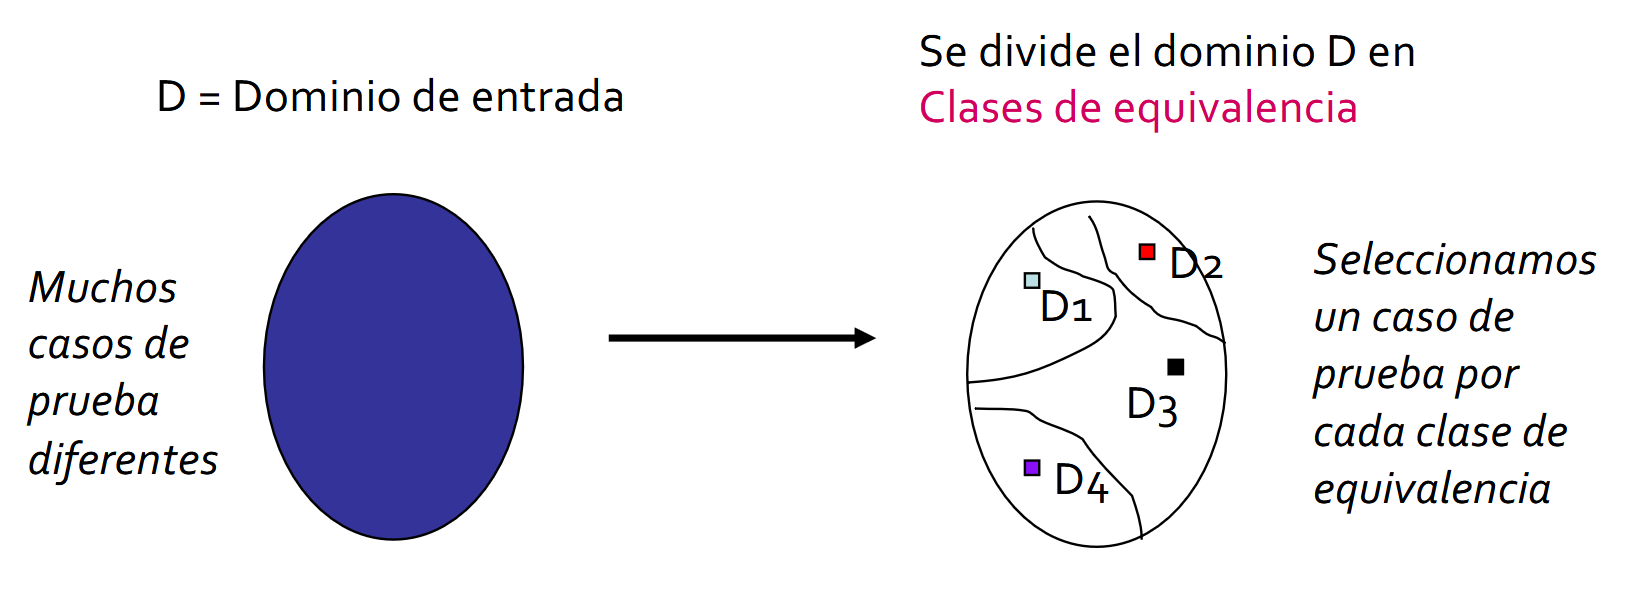
\includegraphics{images/05/claseequivalencia.png}
      \caption{Dividir el dominio}
      \label{fig:05/claseequivalencia}
   \end{figure}
\end{paracol}

Este modelo permite identificar conjuntos de pruebas de tamaño manejable seleccionando unos pocos casos de prueba para cada clase de equivalencia.
Permite también medir la efectividad de la prueba en términos de cobertura relacionada con el modelo de partición creado.
Además, el proceso de partición obliga al tester a pensar sistemáticamente sobre lo que importa

\begin{figure}[htbp]
   \centering
   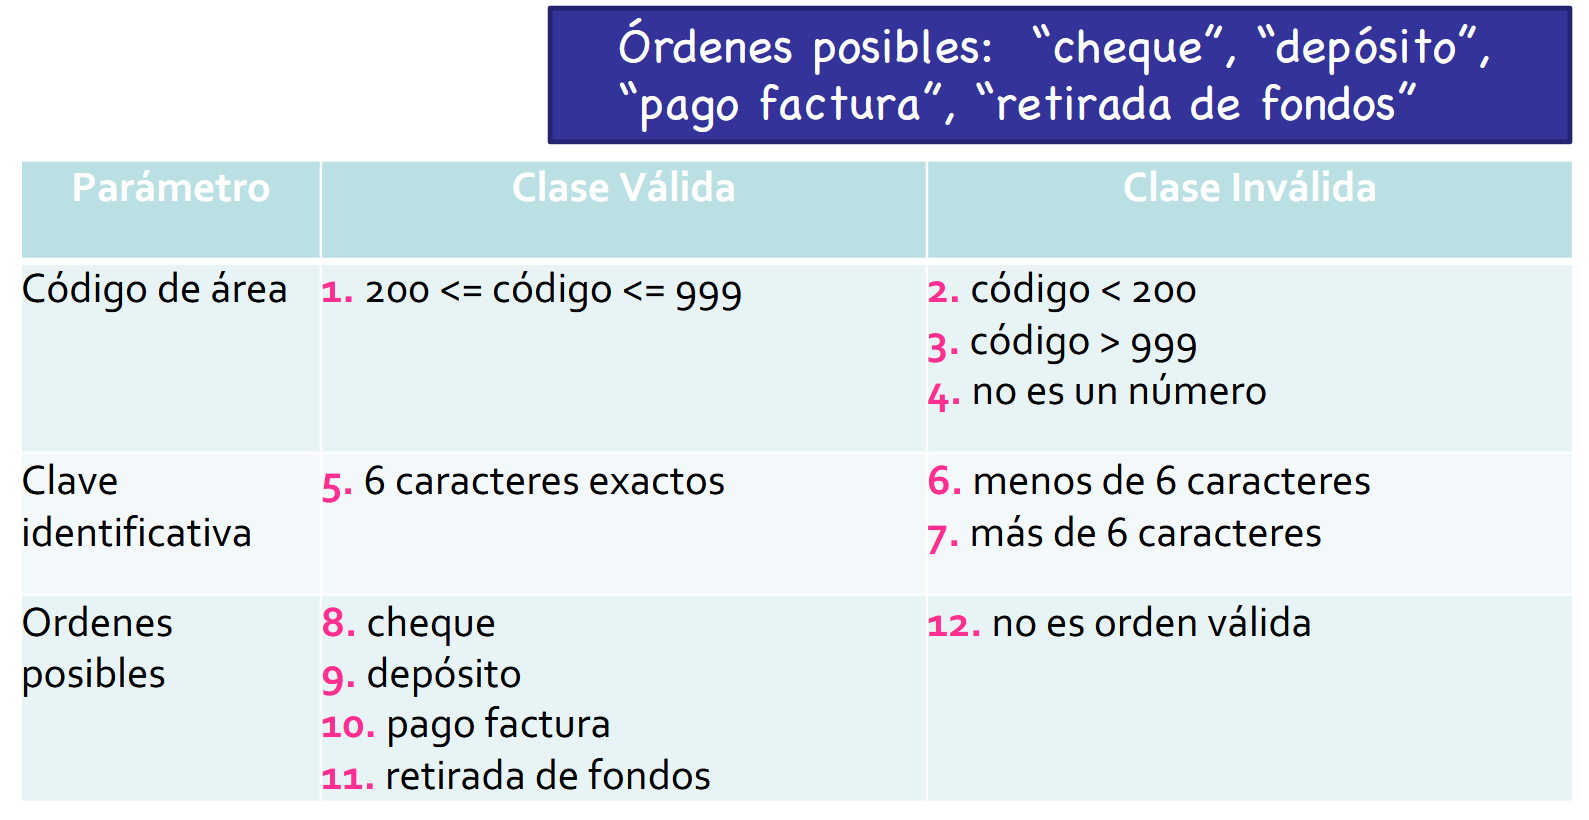
\includegraphics{images/05/claseBanca.png}
   \caption{Ejemplo de una aplicación bancaria}
   {Los datos de entrada son:\ns
   \begin{itemize}
   	\item Código de area: número de tres dígitos que no empieza ni por 0 ni por 1
	\item Clave identificativa de la operación: 6 caracteres alfanuméricos
	\item Órdenes posibles: ``cheque'', ``depósito'', ``pago factura'' , ``retirada de fondos'' 
   \end{itemize}}
   \label{fig:05/claseBanca}
\end{figure}

Es importante enumerar las clases de equivalencia, y no mezclarlas sobre todo.
Cuando se va a escribir las pruebas, cada prueba tiene que ser relacionada con una o más clases de equivalencia, y tenemos que indicar a cuales.

\begin{table}[htbp]
   \centering
   \begin{tabular}{|c|c|c|}
   \hline
       Parámetro & Clase Válida & Clase Inválida \\ \hline
       Capital & $c > min$ & $c \leq min$ \\ \hline
       Ingreso & $i \geq 0$ & $i < 0$ \\ \hline
       Deuda & $d \geq 0$ & $d < 0$ \\ \hline
       Impagados & $T \vee F$ & \\ \hline
       \multirow{4}{*}{Impagados $\wedge$ cond} & 1) $T \wedge (i - d) < c/3$  & ~ \\
       & 2) $F \wedge (i - d) \geq c/3$ & \\
       & 3) $T \wedge (i - d) \geq c/3$ & \\
       & 4) $F \wedge (i - d) < c/3$ & \\ \hline
   \end{tabular}
   \caption{Ejemplo de clases de equivalencia para una aplicación bancaria}
   \note{
   \begin{itemize}
   	\item si el cliente está en una lista de impagados y el sueldo bruto menos la deuda
   	      es inferior al capital solicitado dividido entre 3, la solicitud pasa a No
   	      Concedida.
   	\item si el cliente no está en ninguna lista, y el sueldo bruto menos la deuda es
   	      mayor o igual al capital solicitado dividido entre 3, se clasifica como Pre-
   	      concedida.
   	\item en cualquier otro caso pasa a En estudio
   \end{itemize}
   }
   \label{tab:05/claseEquivalencia}
\end{table}

\section{Tablas de decisión}

Se puede utilizar para programas que toman decisiones basadas en condiciones lógicas sobre combinaciones de entradas, parámetros y/o variables, eligiendo diferentes acciones o respuestas.
\note{\begin{itemize}
	\item La acción o respuesta que se toma no depende del orden en que
se evalúa los valores de los parámetros y variables.
	\item La acción o respuesta que se toma no depende de entradas o
salidas anteriores
\end{itemize}}

\begin{paracol}{2}
   \begin{itemize}
   	\item Cada condición corresponde a una variable, relación o predicado
	\item Valores posibles para las ``Condition Entries''
 \begin{itemize}
 	\item Booleano (\lstinline|True / False|) - Tabla de decisión de entrada limitada
	\item Valores - Tabla de decisión de entrada extendida
	\item Valor ``No Importa'' (Don't care value)

 \end{itemize}
\item Cada acción es una operación que hay que ejecutar

   \end{itemize}
\switchcolumn
\begin{figure}[htbp]
   \centering
   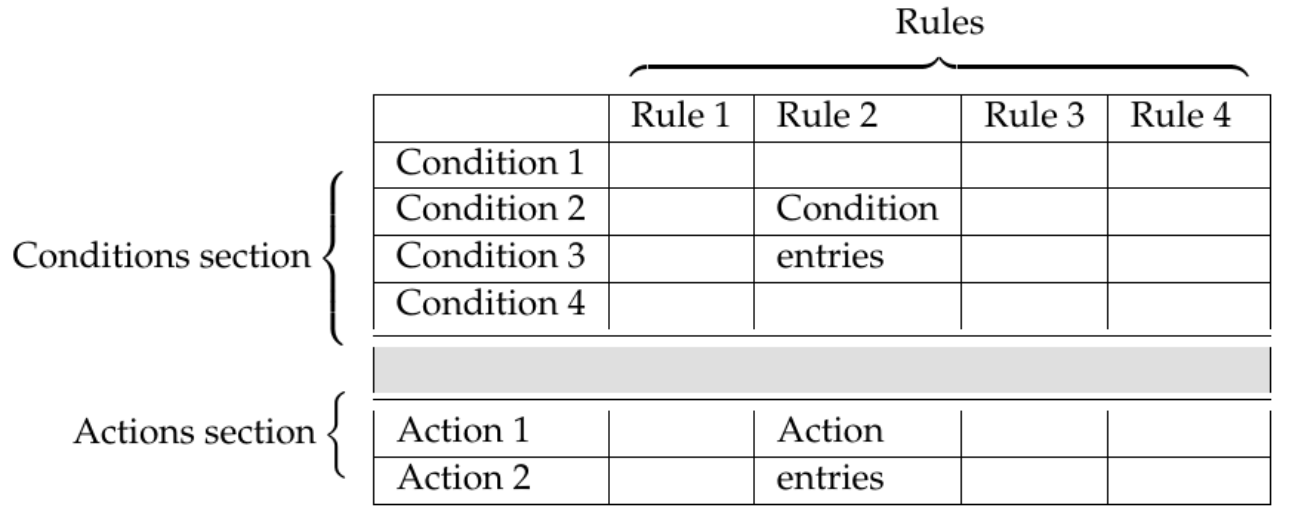
\includegraphics{images/05/tabladecision.png}
   \caption{Tabla decision }
   \label{fig:05/tabladecision}
\end{figure}
\end{paracol}

\begin{figure}[htbp]
   \centering
   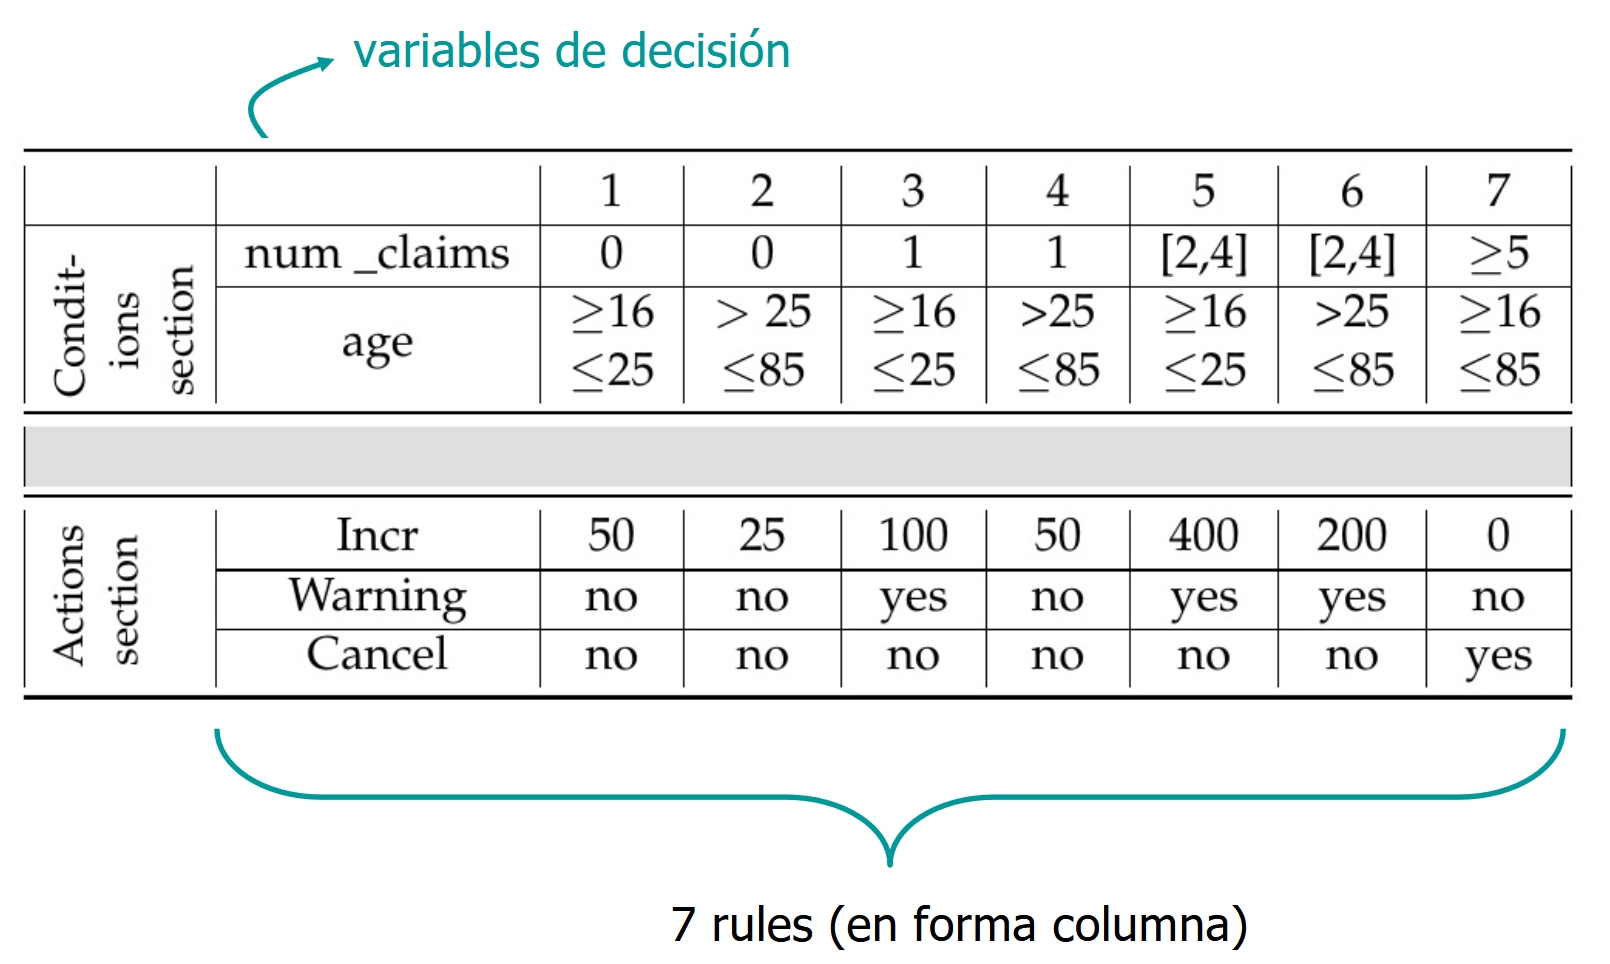
\includegraphics{images/05/tablaForma1.png}
   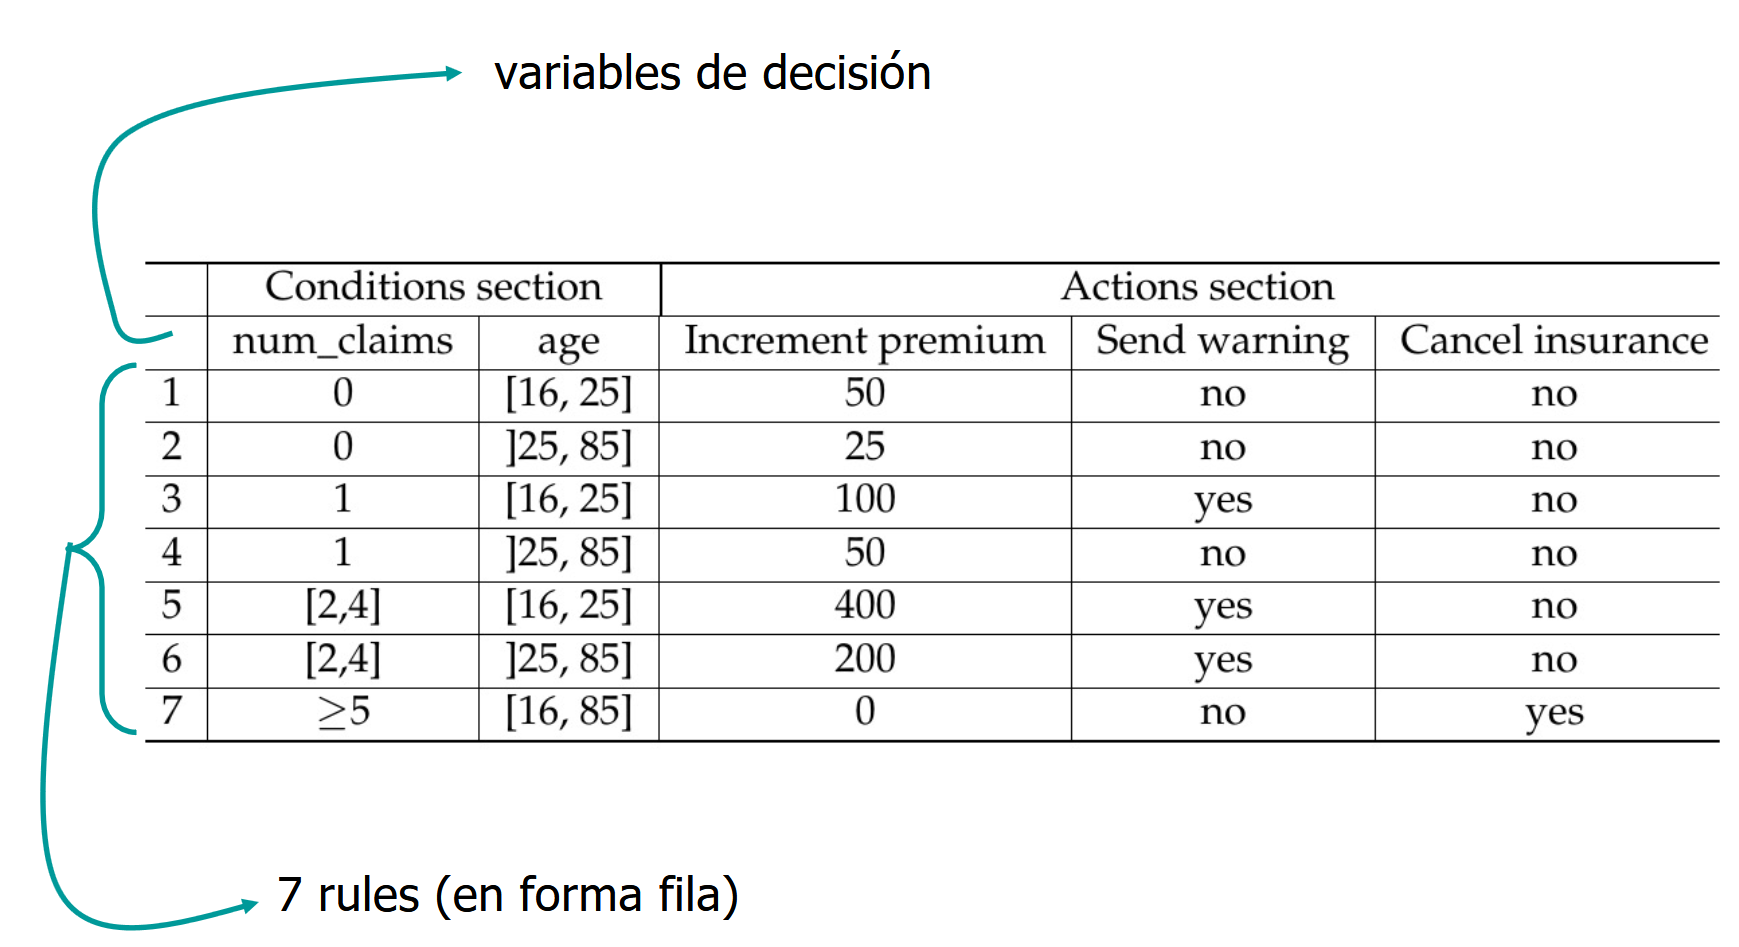
\includegraphics{images/05/tablaForma2.png}
   \caption{Forma columna y forma fila de tablas de decisión}
   \label{fig:05/tablaForma}
\end{figure}

\section{Valores Límites}
\begin{itemize}
	\item Intervalo: un subconjunto del espacio de los valores de entrada de
un programa.
	\item Punto límite de un intervalo (boundary) : aquel punto que según
sea incrementado o decrementado un valor epsilon infinitesimal
dará como resultado un valor perteneciente o no a dicho intervalo.
	\item Desigualdad del límite : una expresión algebraica con $>$, $<$, $\geq$, $\leq$
que define parte de los puntos que pertenecen a un intervalo o
dominio.
	\item Condiciones de igualdad : una expresión algebraica con $=$, $\neq$
\end{itemize}

\begin{figure}[htbp]
   \centering
   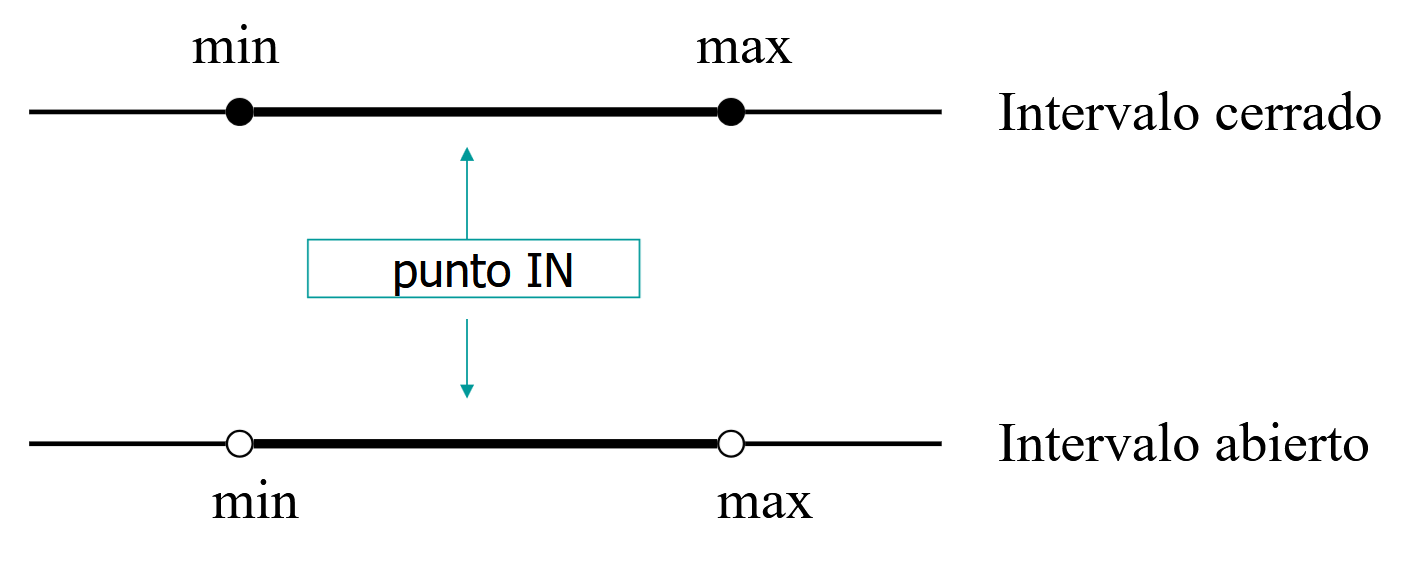
\includegraphics[width=0.45\columnwidth]{images/05/puntoIN.png}
   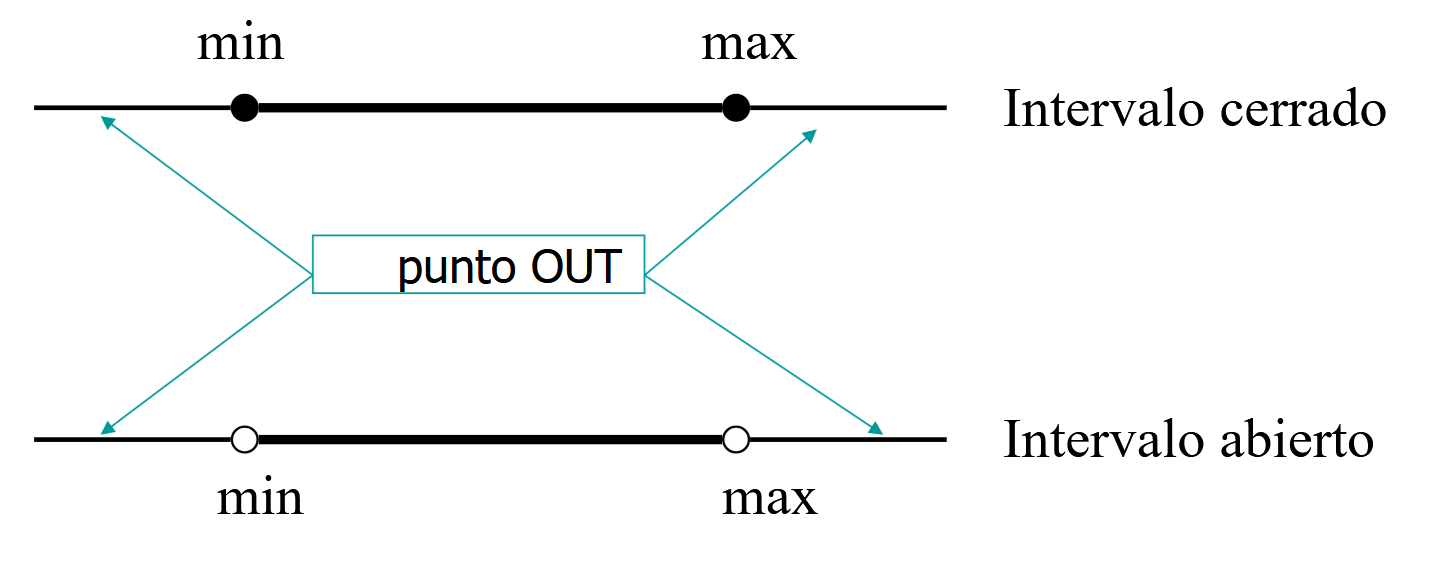
\includegraphics[width=0.45\columnwidth]{images/05/puntoOUT.png}
   \caption{puntoINOUT}
   \label{fig:05/puntoINOUT}
\end{figure}
\begin{figure}[htbp]
   \centering
   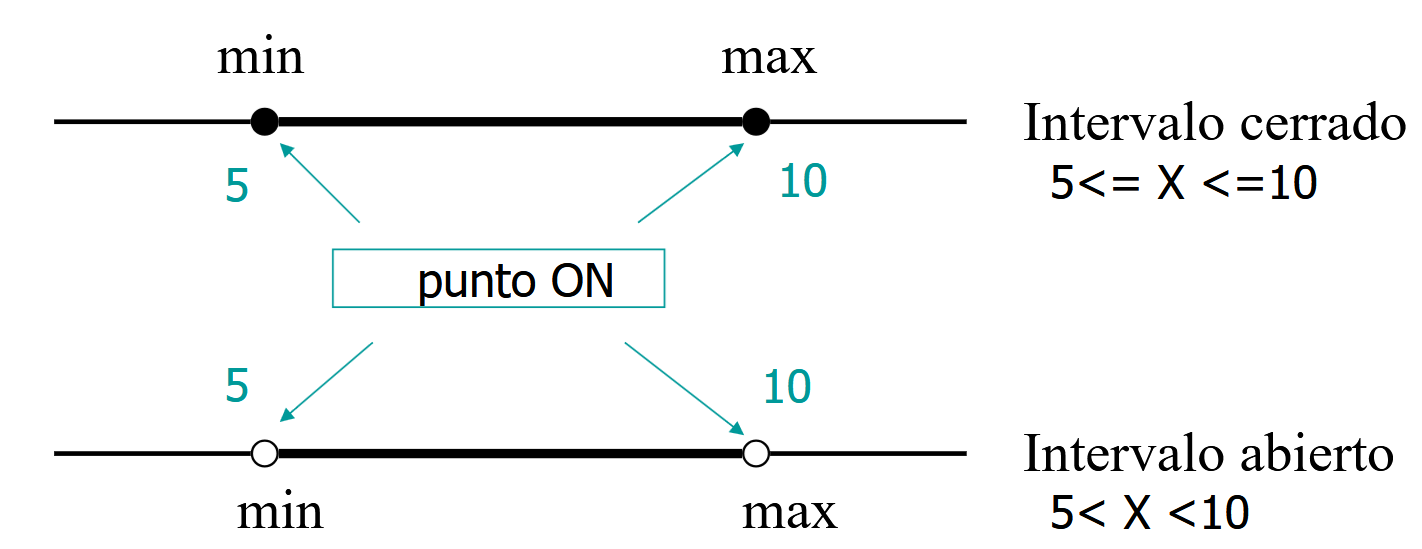
\includegraphics[width=0.45\columnwidth]{images/05/puntoON.png}
   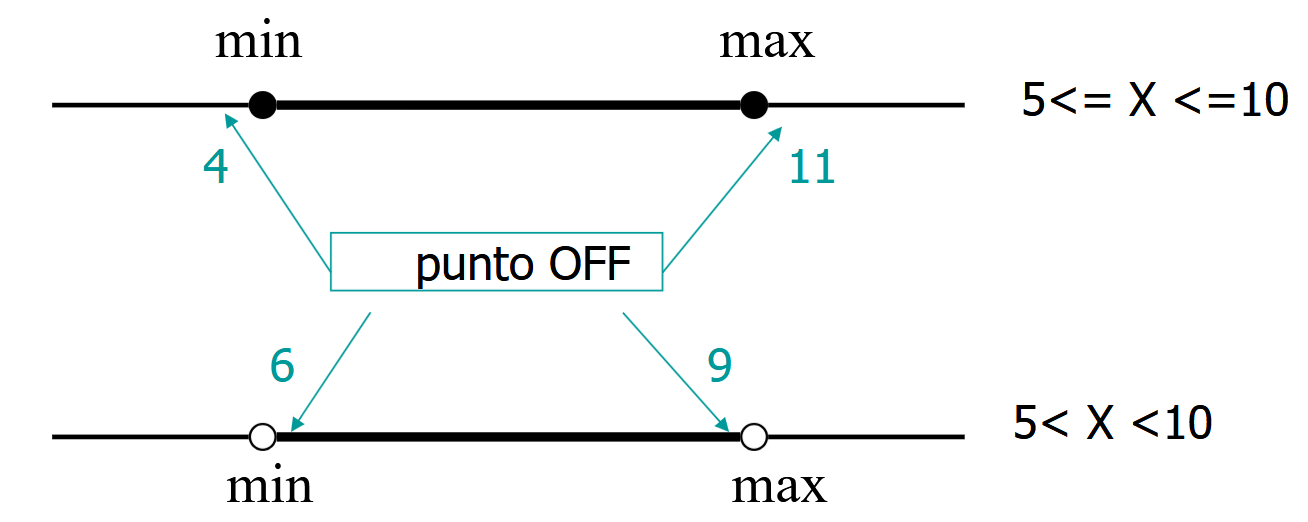
\includegraphics[width=0.45\columnwidth]{images/05/puntoOFF.png}
   \caption{puntoONOFF}
   \label{fig:05/puntoONOFF}
\end{figure}

\begin{itemize}
   \item \textsc{Punto IN} : un punto que pertenece al intervalo
   \item \textsc{Punto OUT} : un punto que no pertenece al intervalo
   \item \textsc{Punto ON} : un punto que pertenece al intervalo y es un límite
   \item \textsc{Punto OFF} : un valor cerca del punto límite de un intervalo
\end{itemize}

La estrategia para diseñar las pruebas de valores límites es 1 punto ON + 1 punto OFF para cada desigualdad de límite.
\note{Ejemplos:
\begin{itemize}
	\item 3 <= extras < 10
	      \begin{itemize}
		      \item Puntos ON: extras = 3; extras = 10
		      \item Puntos OFF: extras = 2; extras = 9
	      \end{itemize}
	\item 2000 < precio\_base <= 5000
	      \begin{itemize}
		      \item Puntos ON?
		      \item Puntos OFF?
	      \end{itemize}
\end{itemize}}

